% Options for packages loaded elsewhere
\PassOptionsToPackage{unicode}{hyperref}
\PassOptionsToPackage{hyphens}{url}
%
\documentclass[
]{article}
\usepackage{amsmath,amssymb}
\usepackage{iftex}
\ifPDFTeX
  \usepackage[T1]{fontenc}
  \usepackage[utf8]{inputenc}
  \usepackage{textcomp} % provide euro and other symbols
\else % if luatex or xetex
  \usepackage{unicode-math} % this also loads fontspec
  \defaultfontfeatures{Scale=MatchLowercase}
  \defaultfontfeatures[\rmfamily]{Ligatures=TeX,Scale=1}
\fi
\usepackage{lmodern}
\ifPDFTeX\else
  % xetex/luatex font selection
\fi
% Use upquote if available, for straight quotes in verbatim environments
\IfFileExists{upquote.sty}{\usepackage{upquote}}{}
\IfFileExists{microtype.sty}{% use microtype if available
  \usepackage[]{microtype}
  \UseMicrotypeSet[protrusion]{basicmath} % disable protrusion for tt fonts
}{}
\makeatletter
\@ifundefined{KOMAClassName}{% if non-KOMA class
  \IfFileExists{parskip.sty}{%
    \usepackage{parskip}
  }{% else
    \setlength{\parindent}{0pt}
    \setlength{\parskip}{6pt plus 2pt minus 1pt}}
}{% if KOMA class
  \KOMAoptions{parskip=half}}
\makeatother
\usepackage{xcolor}
\usepackage[margin=2.54cm]{geometry}
\usepackage{color}
\usepackage{fancyvrb}
\newcommand{\VerbBar}{|}
\newcommand{\VERB}{\Verb[commandchars=\\\{\}]}
\DefineVerbatimEnvironment{Highlighting}{Verbatim}{commandchars=\\\{\}}
% Add ',fontsize=\small' for more characters per line
\usepackage{framed}
\definecolor{shadecolor}{RGB}{248,248,248}
\newenvironment{Shaded}{\begin{snugshade}}{\end{snugshade}}
\newcommand{\AlertTok}[1]{\textcolor[rgb]{0.94,0.16,0.16}{#1}}
\newcommand{\AnnotationTok}[1]{\textcolor[rgb]{0.56,0.35,0.01}{\textbf{\textit{#1}}}}
\newcommand{\AttributeTok}[1]{\textcolor[rgb]{0.13,0.29,0.53}{#1}}
\newcommand{\BaseNTok}[1]{\textcolor[rgb]{0.00,0.00,0.81}{#1}}
\newcommand{\BuiltInTok}[1]{#1}
\newcommand{\CharTok}[1]{\textcolor[rgb]{0.31,0.60,0.02}{#1}}
\newcommand{\CommentTok}[1]{\textcolor[rgb]{0.56,0.35,0.01}{\textit{#1}}}
\newcommand{\CommentVarTok}[1]{\textcolor[rgb]{0.56,0.35,0.01}{\textbf{\textit{#1}}}}
\newcommand{\ConstantTok}[1]{\textcolor[rgb]{0.56,0.35,0.01}{#1}}
\newcommand{\ControlFlowTok}[1]{\textcolor[rgb]{0.13,0.29,0.53}{\textbf{#1}}}
\newcommand{\DataTypeTok}[1]{\textcolor[rgb]{0.13,0.29,0.53}{#1}}
\newcommand{\DecValTok}[1]{\textcolor[rgb]{0.00,0.00,0.81}{#1}}
\newcommand{\DocumentationTok}[1]{\textcolor[rgb]{0.56,0.35,0.01}{\textbf{\textit{#1}}}}
\newcommand{\ErrorTok}[1]{\textcolor[rgb]{0.64,0.00,0.00}{\textbf{#1}}}
\newcommand{\ExtensionTok}[1]{#1}
\newcommand{\FloatTok}[1]{\textcolor[rgb]{0.00,0.00,0.81}{#1}}
\newcommand{\FunctionTok}[1]{\textcolor[rgb]{0.13,0.29,0.53}{\textbf{#1}}}
\newcommand{\ImportTok}[1]{#1}
\newcommand{\InformationTok}[1]{\textcolor[rgb]{0.56,0.35,0.01}{\textbf{\textit{#1}}}}
\newcommand{\KeywordTok}[1]{\textcolor[rgb]{0.13,0.29,0.53}{\textbf{#1}}}
\newcommand{\NormalTok}[1]{#1}
\newcommand{\OperatorTok}[1]{\textcolor[rgb]{0.81,0.36,0.00}{\textbf{#1}}}
\newcommand{\OtherTok}[1]{\textcolor[rgb]{0.56,0.35,0.01}{#1}}
\newcommand{\PreprocessorTok}[1]{\textcolor[rgb]{0.56,0.35,0.01}{\textit{#1}}}
\newcommand{\RegionMarkerTok}[1]{#1}
\newcommand{\SpecialCharTok}[1]{\textcolor[rgb]{0.81,0.36,0.00}{\textbf{#1}}}
\newcommand{\SpecialStringTok}[1]{\textcolor[rgb]{0.31,0.60,0.02}{#1}}
\newcommand{\StringTok}[1]{\textcolor[rgb]{0.31,0.60,0.02}{#1}}
\newcommand{\VariableTok}[1]{\textcolor[rgb]{0.00,0.00,0.00}{#1}}
\newcommand{\VerbatimStringTok}[1]{\textcolor[rgb]{0.31,0.60,0.02}{#1}}
\newcommand{\WarningTok}[1]{\textcolor[rgb]{0.56,0.35,0.01}{\textbf{\textit{#1}}}}
\usepackage{graphicx}
\makeatletter
\newsavebox\pandoc@box
\newcommand*\pandocbounded[1]{% scales image to fit in text height/width
  \sbox\pandoc@box{#1}%
  \Gscale@div\@tempa{\textheight}{\dimexpr\ht\pandoc@box+\dp\pandoc@box\relax}%
  \Gscale@div\@tempb{\linewidth}{\wd\pandoc@box}%
  \ifdim\@tempb\p@<\@tempa\p@\let\@tempa\@tempb\fi% select the smaller of both
  \ifdim\@tempa\p@<\p@\scalebox{\@tempa}{\usebox\pandoc@box}%
  \else\usebox{\pandoc@box}%
  \fi%
}
% Set default figure placement to htbp
\def\fps@figure{htbp}
\makeatother
\setlength{\emergencystretch}{3em} % prevent overfull lines
\providecommand{\tightlist}{%
  \setlength{\itemsep}{0pt}\setlength{\parskip}{0pt}}
\setcounter{secnumdepth}{-\maxdimen} % remove section numbering
% definitions for citeproc citations
\NewDocumentCommand\citeproctext{}{}
\NewDocumentCommand\citeproc{mm}{%
  \begingroup\def\citeproctext{#2}\cite{#1}\endgroup}
\makeatletter
 % allow citations to break across lines
 \let\@cite@ofmt\@firstofone
 % avoid brackets around text for \cite:
 \def\@biblabel#1{}
 \def\@cite#1#2{{#1\if@tempswa , #2\fi}}
\makeatother
\newlength{\cslhangindent}
\setlength{\cslhangindent}{1.5em}
\newlength{\csllabelwidth}
\setlength{\csllabelwidth}{3em}
\newenvironment{CSLReferences}[2] % #1 hanging-indent, #2 entry-spacing
 {\begin{list}{}{%
  \setlength{\itemindent}{0pt}
  \setlength{\leftmargin}{0pt}
  \setlength{\parsep}{0pt}
  % turn on hanging indent if param 1 is 1
  \ifodd #1
   \setlength{\leftmargin}{\cslhangindent}
   \setlength{\itemindent}{-1\cslhangindent}
  \fi
  % set entry spacing
  \setlength{\itemsep}{#2\baselineskip}}}
 {\end{list}}
\usepackage{calc}
\newcommand{\CSLBlock}[1]{\hfill\break\parbox[t]{\linewidth}{\strut\ignorespaces#1\strut}}
\newcommand{\CSLLeftMargin}[1]{\parbox[t]{\csllabelwidth}{\strut#1\strut}}
\newcommand{\CSLRightInline}[1]{\parbox[t]{\linewidth - \csllabelwidth}{\strut#1\strut}}
\newcommand{\CSLIndent}[1]{\hspace{\cslhangindent}#1}
\usepackage{titling}
\pretitle{\begin{flushright}

\includegraphics[width=2in,height=2in]{logo.png}\LARGE\\}
\posttitle{\end{flushright}}
\usepackage{amsmath}
\usepackage{fancyhdr}
\pagestyle{fancy}
\fancyhead[L]{fabryka}
\fancyhead[R]{R web application for fabric analysis}
\fancyfoot[C]{\thepage}
\usepackage{float}
\floatplacement{figure}{H}
\usepackage{bookmark}
\IfFileExists{xurl.sty}{\usepackage{xurl}}{} % add URL line breaks if available
\urlstyle{same}
\hypersetup{
  pdftitle={ fabryka},
  hidelinks,
  pdfcreator={LaTeX via pandoc}}

\title{\hfill\break
\textbf{fabryka}}
\usepackage{etoolbox}
\makeatletter
\providecommand{\subtitle}[1]{% add subtitle to \maketitle
  \apptocmd{\@title}{\par {\large #1 \par}}{}{}
}
\makeatother
\subtitle{A web application for easily analysing \& exploring the fabric
of archaeological assemblages}
\author{}
\date{\vspace{-2.5em}}

\begin{document}
\maketitle

\renewcommand{\[}{\begin{equation}}
\renewcommand{\]}{\end{equation}}

\textbf{Marc Thomas} \textsuperscript{1*}
(\url{https://orcid.org/0000-0002-8160-1910}) \smallbreak

\textsuperscript{1} TRACES, UMR 5608 - Université Toulouse Jean Jaurès,
5 Allée Antonio Machado, FR-31058 Toulouse Cedex 9 \smallbreak

\textsuperscript{*} Corresponding author \smallbreak

E-mail:
\href{mailto:marcthomas1@hotmail.fr}{\nolinkurl{marcthomas1@hotmail.fr}}
\smallbreak

\textbf{Key words}: R shiny web application, fabric, site formation
processes, spatial analysis, orientation and dip \bigbreak

\section{Abstract}\label{abstract}

This article presents fabryka 1.1, an open access R shiny web
application dedicated to the fabric analysis of archaeological or
geological assemblages. The fabric is a statistic made of the
orientation and dip of elongated particles and archaeological objects.
It provides information about the nature of the geological processes
involved in the formation of the deposits and their impact on the
preservation of the archaeological assemblages. This statistical
analysis is not easily accessible to non-specialists and is particularly
time-consuming, sometimes requiring the use of several software, some of
which are chargeable. fabryka uses classical analytical procedures
(Benn, rose, Schmidt and Woodcock diagrams and statistical tests on
orientations) for analysing the fabrics of objects and includes a
spatial method. New statistical methods and new ways of exploration are
proposed in the application and in this present article.\smallbreak

You can use fabryka by following this link
\url{https://marchaeologist.shinyapps.io/fabryka/} or by launching the
application in Rstudio thanks to its script. The fabryka application
files, made in R (\citeproc{ref-rcoreteam2025}{Team 2025}) by using the
R package \emph{shiny} (\citeproc{ref-chang2024}{Chang et al. 2024}),
and this article, written in rmarkdown
(\citeproc{ref-allaire2014}{Allaire et al. 2014};
\citeproc{ref-xie2018}{Xie, Allaire, and Grolemund 2018};
\citeproc{ref-xie2020}{Xie, Dervieux, and Riederer 2020}), are both
available online in a public github repository
(\url{https://github.com/marchaeologist/fabryka/tree/main}). \pagebreak

\section{Introduction}\label{introduction}

Fabric is made of the orientation and dip of elongated objects
(\citeproc{ref-bertran1997}{Bertran et al. 1997};
\citeproc{ref-bertran2002}{Bertran and Lenoble 2002};
\citeproc{ref-lenoble2004}{Lenoble and Bertran 2004}). It is a statistic
(\emph{i.e.}, it needs as much measurements as possible) that enables
the identification of sedimentary processes involved in the formation of
the deposits (\citeproc{ref-bertran1997}{Bertran et al. 1997};
\citeproc{ref-bertran2002}{Bertran and Lenoble 2002};
\citeproc{ref-lenoble2004}{Lenoble and Bertran 2004}) and their impact
on archaeological assemblages (\citeproc{ref-isaac1967}{Isaac 1967};
\citeproc{ref-schick1986}{Schick 1986}; \citeproc{ref-thomas2019}{Thomas
et al. 2019}). Objects abandoned by prehistoric people can be considered
as sedimentary particles and are affected by natural processes
(\citeproc{ref-schiffer1983}{Schiffer 1983}). As geological particles
are often not elongated enough, analysis of the fabric of sedimentary
deposits often depends mainly on archaeological material (bones and
lithics). This makes it possible to identify the sedimentary processes
to which they were subjected and to discuss their degree of spatial
reorganization. When possible, distinguishing sedimentary particles from
archaeological objects in the fabric analysis could allow to test
whether these two populations were affected by different processes
(\emph{e.g.}, the fabric of an undisturbed occupation covered by
deposits from a minor flood should reveal a distinct fabric from that of
the alluvial pebbles on which it rests).

One of the first archaeological application probably dates to the
experiments carried out by the South African G. Isaac (1967) on the
shores of Lake Magadi in Kenya. G. Isaac wanted to explain the role
played by hydrological processes on the bone accumulations found in the
Great Rift Valley. In November 1964, he placed several concentrations of
experimental material near a river branch. A few months later, heavy
rains had reactivated the valley's rivers. In addition to the
displacement or even loss of all or part of the material, G. Isaac
revealed a reorientation that was mainly perpendicular and, to a lesser
extent, parallel to the orientation of flow, with a slight upstream dip.
Since G. Isaac's pioneering work, there has been an abundant literature
devoted to the analysis of fabrics (\citeproc{ref-benn1994}{Benn 1994};
\citeproc{ref-lenoble2004}{Lenoble and Bertran 2004};
\citeproc{ref-mcpherron2018}{S. P. McPherron 2018}) allowing this method
to be increasingly performed on archaeological sites.

Numerical methods have been developed to measure the orientation and dip
of objects in the field (\citeproc{ref-mcpherron2005artifact}{S. J.
McPherron 2005}; \citeproc{ref-discamps2024}{Discamps et al. 2024}) or
from field archives such as plans and photos
(\citeproc{ref-de2013application}{Torre and Benito-Calvo 2013};
\citeproc{ref-sanchez2016assessment}{Sánchez-Romero et al. 2016}).

Two main families of statistical method are commonly used to
characterize the fabric of a given assemblage
(\citeproc{ref-bertran2002}{Bertran and Lenoble 2002};
\citeproc{ref-mcpherron2018}{S. P. McPherron 2018};
\citeproc{ref-de2021new}{Torre et al. 2021}). \newline The first methods
focus on the orientation only and aim to test the null hypothesis of a
random orientation of objects through several statistical tests
(\citeproc{ref-krumbein1939}{Krumbein 1939};
\citeproc{ref-curray1956}{Curray 1956}; \citeproc{ref-rao1967large}{Rao
1967}).\newline The second statistical method takes into account object
orientation and dip. Three normalized eigenvalues (E1, E2 and E3) are
calculated from the cosine formed by the axis of the artifact with the
three axes of space (\citeproc{ref-watson1966}{Watson 1966}). Woodcock
(\citeproc{ref-woodcock1977}{1977}) and Benn
(\citeproc{ref-benn1994}{1994}) indices are used to describe the fabric
shape. Several authors \emph{e.g.}, (\citeproc{ref-bertran1997}{Bertran
et al. 1997}; \citeproc{ref-bertran2002}{Bertran and Lenoble 2002};
\citeproc{ref-lenoble2004}{Lenoble and Bertran 2004}) built models to
compare the fabric of archaeological assemblages to natural sedimentary
processes and human processes (\emph{i.e.}, fabric of knapping spots).
The null hypothesis of an absence of perturbation is a fabric shape
compatible with that of experimental knapping spots. These methods are
described in the Mathematics section of this article.

Several software allow data processing, some of which are not freely
accessible, do not allow spatial exploration of the data or do not offer
interfaces to facilitate the task of non-programmer users
(\citeproc{ref-mcpherron2018}{S. P. McPherron 2018}). The following
sections explain all the selected approaches and our proposals for
processing the fabrics thanks to fabryka, from taking measurements in
the field, through the statistical methods and graphical modes of
representation used in the application
(fig.~\ref{fig:figure_presentation}). \bigbreak

\begin{figure} [h]
\centering
  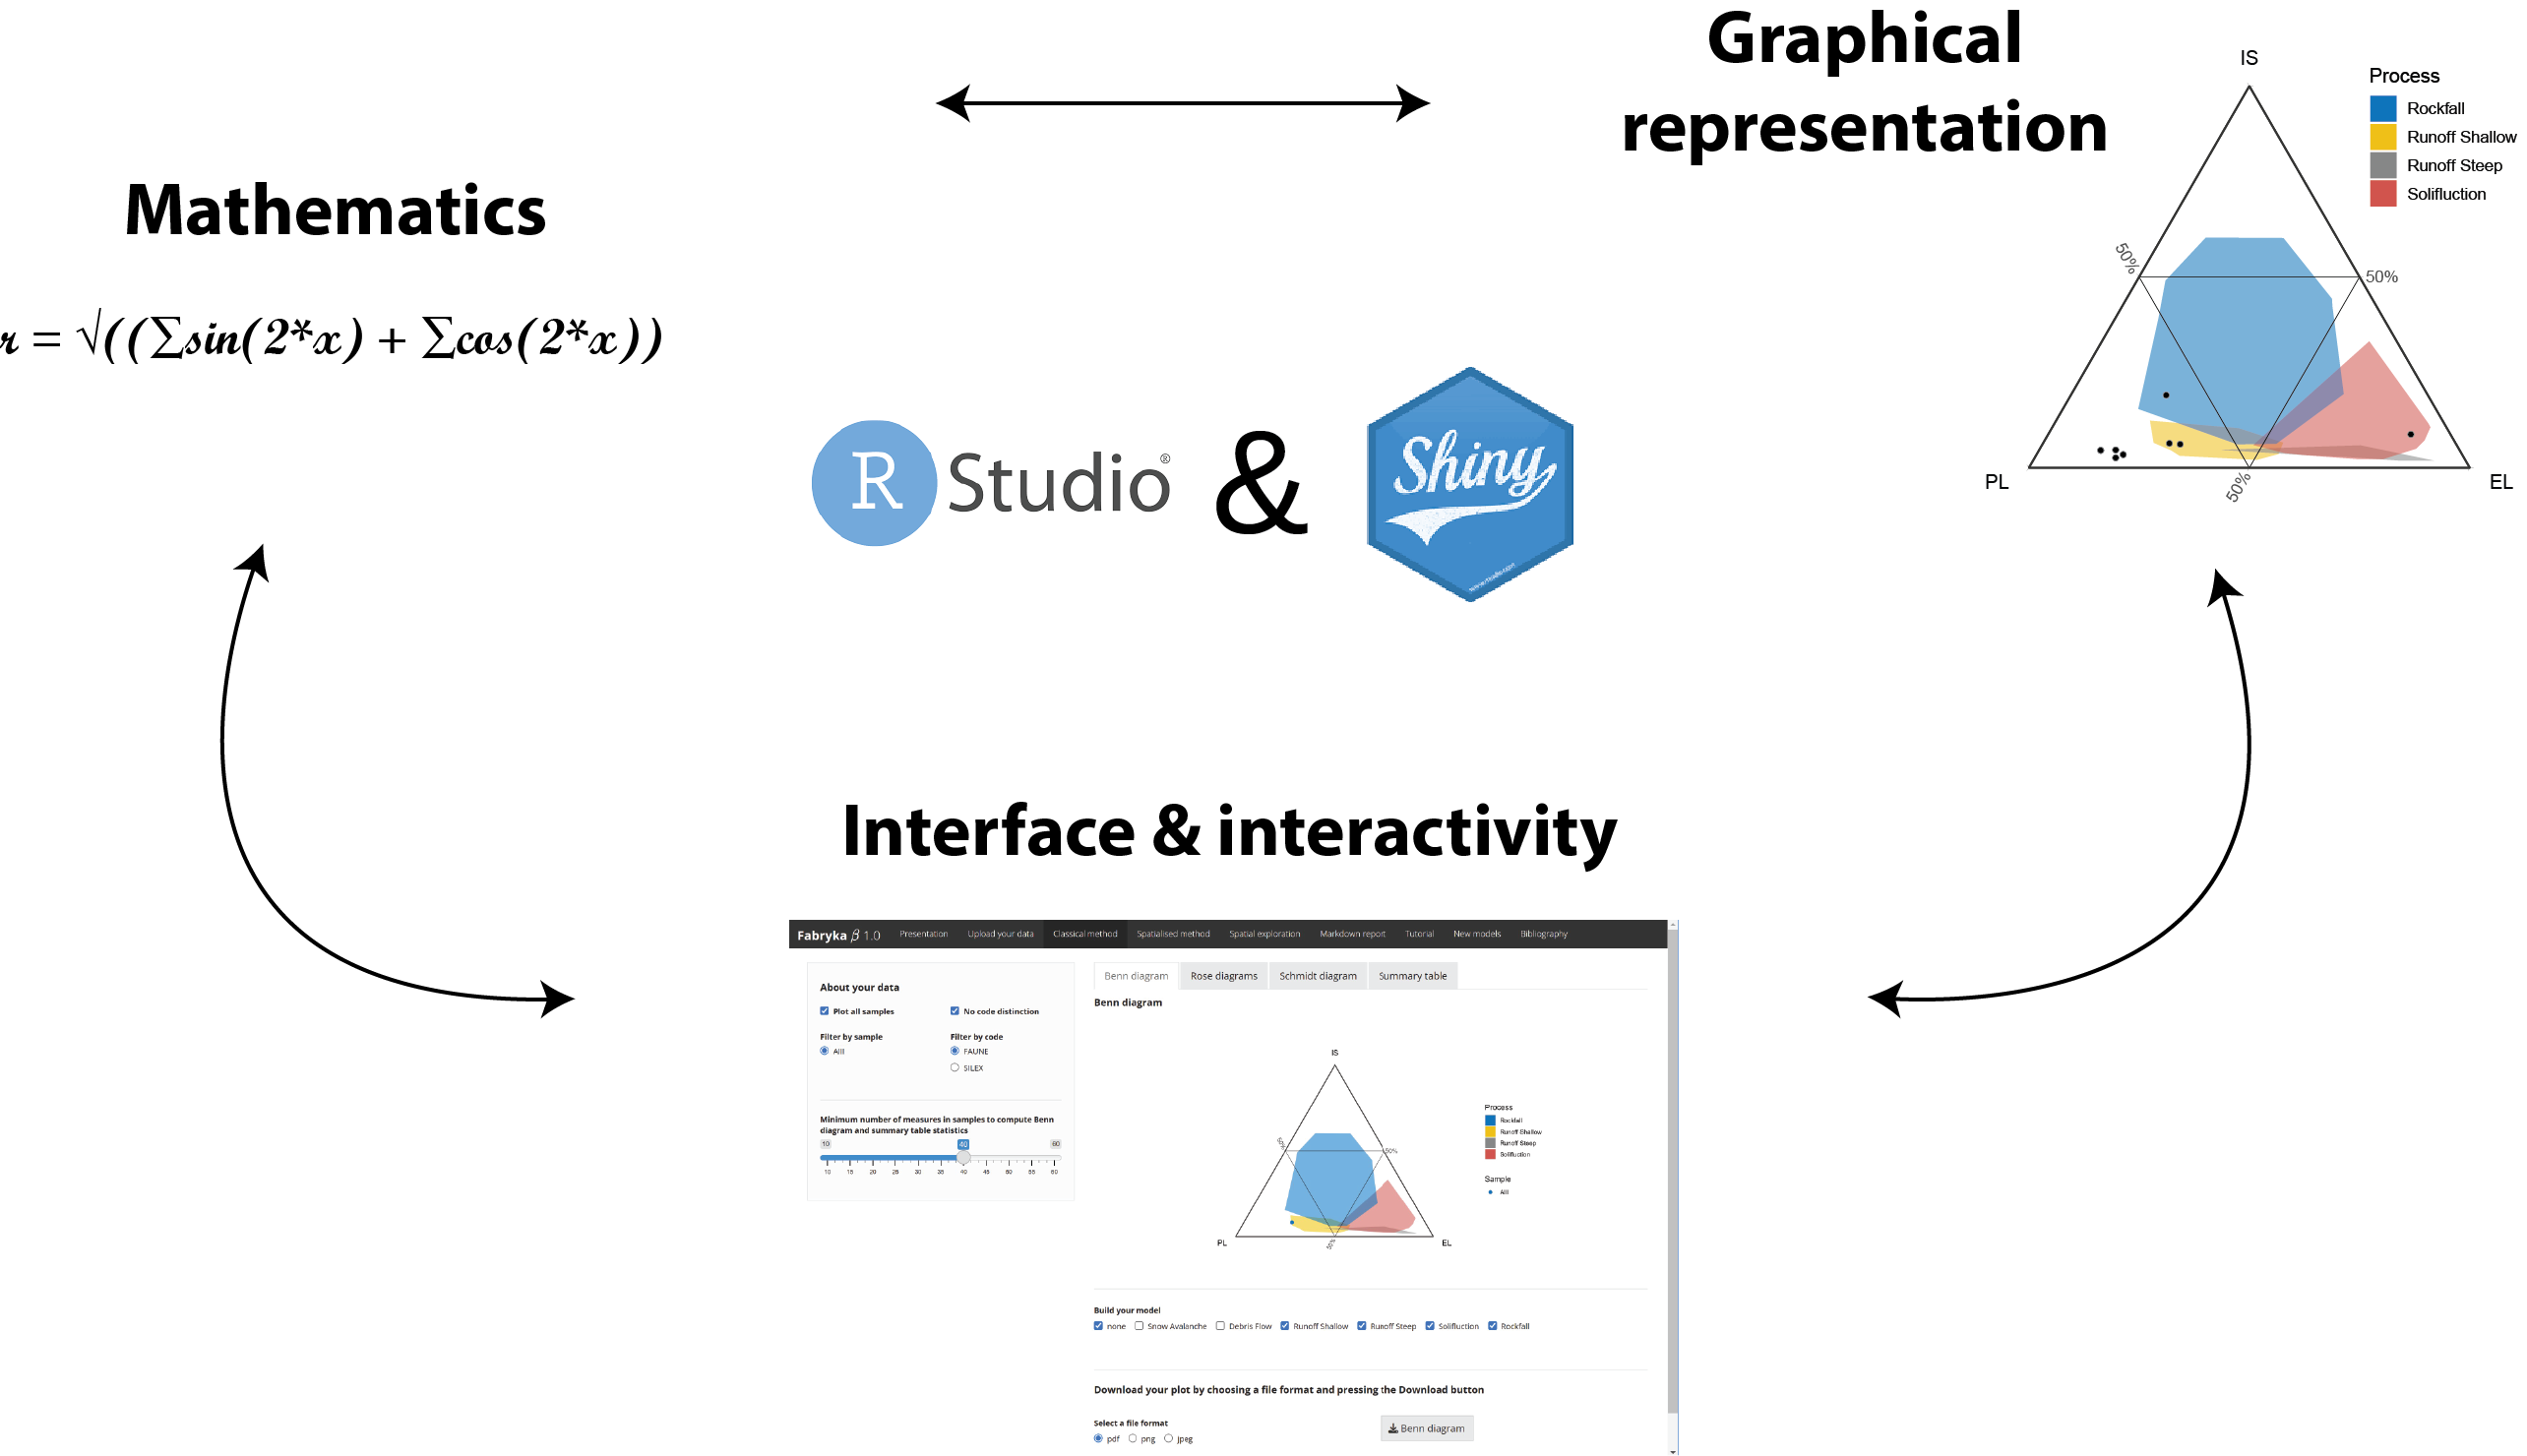
\includegraphics[width=15cm]{figure/presentation_applications.png}
  \caption{fabryka creation scheme and organisation of the article}
\label{fig:figure_presentation}
\end{figure}

\section{Field data acquisition}\label{field-data-acquisition}

During excavation, the orientation and dip of elongated remains
(\emph{i.e.} a \textgreater{} 2 * b and with a \textgreater{} 2 cm) is
measured on a representative set of artefacts or on the whole
assemblage. The orientation (= bearing) of the lowest point is measured
in the range {[}0; 360{[} with North as the reference (\emph{i.e.}
orientation = 0°). The dip (= plunge) is measured in the range {[}0;
90{]} with horizontal as a reference. The orientation {[}0; 360{[} can
be converted into axial data measured in the range {[}0; 180{[} by
subtracting 180° from the measurements in the range {[}180; 360{]}.

Traditionally, the azimuth of the principal axis of an object is
measured using a compass considering that the point with the lowest
altitude indicates the orientation of the vector. The dip is measured
using an inclinometer. The aim is to measure the orientation and dip of
the elongaton axis of of objects ignoring its shape. To do this, the
measuring device must be placed parallel to the elongation axis of the
object. Measuring the fabric from its imprint or visible surface is
biased by its shape, making impossible to assess its true dip. Since the
theodolite was introduced to excavations in the 1990s, the fabrics is
sometimes measured by recording the coordinates of the ends of objects
(\citeproc{ref-mcpherron2005artifact}{S. J. McPherron 2005}). In the
latter case, the rules of trigonometry are applied to convert the pair
of coordinates into orientations and dips.

Recently, speleologist have created a digital inclinometer (Leica
DistoX310 modified to DistoX2; \url{https://paperless.bheeb.ch/}) which
can be used to measure fabrics (\citeproc{ref-discamps2024}{Discamps et
al. 2024}). The device stores and associates data with the order of
measurement. When the device is tilted downwards, the orientation of the
lowest point is measured and, the recorded dip is negative. When the
device is tilted upwards, the orientation of the highest point is
recorded, and the dip is positive. To obtain data that is suitable for
statistical analysis, in the first case the absolute value of the dip
must be retained. In the second case (\emph{i.e.} positive dip), if the
measured orientation is in the interval {[}0; 180{]}, 180° must be added
to the orientation, and if the measured orientation is in the interval
{]}180; 360{]}, 180° must be subtracted from the orientation.

When possible, preferring the use of a digital inclinometer avoids many
errors during measurement and data recording. On the other hand, for the
reasons given above, the use of a theodolite to measure fabrics is not
recommended as it results in inaccurate dip measurements. As well,
measuring orientations and dip in sections leads to sampling biases.

A sample corresponds to all the orientation and dip measurements taken
within a Lithostratigraphic Unit (LU) or a pedostratigraphic unit. These
units seem to be the most coherent entity which needs to be explored
because they are defined according to geological criteria, which a
priori guarantee a certain coherence in terms of the formation dynamics
we are seeking to approach. In fabryka, analysis are constrained within
samples unless the user decides otherwise in the spatial exploration
panel. \bigbreak

\section{Mathematics}\label{mathematics}

\subsection{Classical method}\label{classical-method}

Two main statistical family methods are used:

\begin{enumerate}
\def\labelenumi{\arabic{enumi}.}
\tightlist
\item
  The first considers the orientation only. The calculation of the
  Vector Magnitude \(L\) (expressed as a percentage) by Curray's
  (\citeproc{ref-curray1956}{1956}) formula tests the hypothesis of an
  unimodal distribution of orientations. If the \(p\) value returned by
  the Rayleigh test is less than the threshold of 0.05, the null
  hypothesis of a random sampling from a uniform distribution is
  rejected. The formula for calculating the Vector Magnitude \(L\) is as
  follows:
\end{enumerate}

Curray's formula to calculate \(L\) is:

\[L = \frac{r*100}{n}\] with:

\[r = \sqrt{\sum_{i=\alpha}^n \sin{(2\alpha)} + \sum_{i=\alpha}^n \cos{(2\alpha)}}\]
\smallbreak where \(n\) is the number of measures and \(\alpha\), is the
axial data (0 to 180°) \smallbreak

The Rayleigh test is performed thanks to the formula:

\[p = e^{(-(n*L^2))*10^-4}\]

The method consisting of doubling the value of the axial angles before
calculating the Vector Magnitude \(L\) and the Rayleigh test, as
proposed by Krumbein (\citeproc{ref-krumbein1939}{1939}), tests the
hypothesis of a bimodal distribution with a period of 90°. The
hypothesis of a 90° period bimodal distribution of a sample of
orientations is retained when \(p\) \textless0.05
(\citeproc{ref-curray1956}{Curray 1956}). The sensitivity of the
Rayleigh test to the sample size \(n\) prevents samples from being
compared with each other when \(n\) varies
(\citeproc{ref-curray1956}{Curray 1956};
\citeproc{ref-bertran2002}{Bertran and Lenoble 2002}). For example, when
the Vector Magnitude \(L\) is 25\%, the Rayleigh test gives \(p-values\)
below a critical threshold of 0.05 for series with more than 50
measurements (fig.~2).

The Rao (\citeproc{ref-rao1967large}{1967}) spacing test assesses the
uniformity of circular data. It determines whether the data show
significant directionality (\emph{i.e.} the null hypothesis is a uniform
distribution). It is widely used to detect multimodal directionality.

\begin{enumerate}
\def\labelenumi{\arabic{enumi}.}
\setcounter{enumi}{1}
\tightlist
\item
  The second considers the orientation and dip of the objects. The
  normalised eigenvalues \(E1\), \(E2\) and \(E3\) are calculated from
  the cosine formed by the axis of the objects with the three axes of
  space (\citeproc{ref-watson1966}{Watson 1966}).
\end{enumerate}

The fabric shape can be described by calculating the ratios \(r1\) =
ln(E1/E2), \(r2\) = ln(E2/E3) and \(K\) = r1/r2
(\citeproc{ref-woodcock1977}{Woodcock 1977}). When 0 \textless{} \(K\)
\textless{} 1, the fabric is planar. When 1 \textless{} \(K\)
\textless{} \(+\infty\), the fabric is linear. The parameter \(C\) =
ln(E1/E3) is a measure of the strength of the preferred orientation
(\citeproc{ref-woodcock1977}{Woodcock 1977}). These indices can be
plotted into a Woodcock diagram.

The Benn indices (\citeproc{ref-benn1994}{Benn 1994}) describe the
fabric shape of a sample and can be plotted in a ternary diagram
(\emph{i.e.} Benn diagram). The elongation index EL is equal to
\(1-(E2/E1)\) and the isotropy index \(IS\) is \(E3/E1\). When \(EL\) is
high, the axes of the objects are grouped around an orientation. When
\(IS\) is high, the fabric is said to be isotropic meaning the axes of
the objects are uniformly distributed in all directions. Finally, when
the value \(1-EL-IS\) is high, the fabric is said to be planar, with the
axes of the objects grouped around a plane. \bigskip

\begin{figure}
\centering
\pandocbounded{\includegraphics[keepaspectratio]{article_files/figure-latex/rayleigh-1.pdf}}
\caption{Evolution of the p-value returned by the Rayleigh test as a
function of the Vector Magnitude `L' and the sample size `n'
\label{rayleigh}}
\end{figure}

\subsection{Spatialised method}\label{spatialised-method}

To distinguish different statistical populations, a spatial method
proposed by McPherron (\citeproc{ref-mcpherron2018}{2018}) is used.
Thanks to this method it is possible to calculate the Benn indices and
the Vector Magnitude \(L\) (formula (\textbf{3.}) modified from
McPherron (\citeproc{ref-mcpherron2018}{2018}) R script) for each
remains, and its \(n\) nearest neighbors in 3 dimensions (McPherron
(\citeproc{ref-mcpherron2018}{2018}) R script, modified, formula
(\textbf{4.})). The analysis of the fabric as proposed by McPherron
(\citeproc{ref-mcpherron2018}{2018}) has the advantage of spatialising
the measurements. It is possible to localize the statistical signal of
fabrics by varying the number of measurements sampled to calculate the
Benn indices. The choice of about 40 to 60 measurements (each remain and
its 40 to 60 nearest neighbors) to calculate the Benn indices allows
local particularities to be observed, and above all, it allows the
Rayleigh test to be carried out in its field of application (stability
of the test between around 40 to 50 measurements after Bertran and
Lenoble (\citeproc{ref-bertran2002}{2002})).

By avoiding the instability of the Rayleigh test, the rejection rate
\(Tr\) of the null hypothesis provides a more reliable description of
the distribution of orientations in a sample. In addition, it allows
comparisons between samples despite varying sample size.

The rejection ratio \(Tr\) is performed thanks to the formula:

\[Tr = \frac{(n~times~p.value < 0.05)* 100}{n}\]

\section{Graphical representation}\label{graphical-representation}

Several methods of representation are used. Rose diagrams summaries the
orientation and dip measurements for each sample. Benn indices are
projected in a Benn diagram and measures (orientation and dip) are
projected into Schmidt diagrams. These figures are available for both
`classical' and `spatialised' methods.

As submited by S. P. McPherron (\citeproc{ref-mcpherron2018}{2018}), a
spatial investigation of the fabric is proposed in a dedicated panel.
Benn (\citeproc{ref-benn1994}{1994}) indices calculated for each spatial
series of remains are projected within a Benn diagram in which each pole
(isotropic, linear, and planar) is colored respectively in red, green
and blue. The RGB color code is reused to materialize the fabric of the
remains on spatial projections (plan and section views) of the material
along the axes of the excavation grid. \bigbreak

\section{Interface and user
interactivity}\label{interface-and-user-interactivity}

The next sections provide a description and a tutorial of fabryka. All
the figures in this section were produced using the example data set
provided in the application (\emph{i.e.} ``Case 3: Angles from DistoX2
with coordinates).''

\subsection{Upload data}\label{upload-data}

The simplest method to upload data in the application is to name the
column names directly, as shown in the example files. Enter your data in
a csv file, adding the columns `id', `code' and `sample'. If the columns
don't exist, fill them in with the same letter. By doing so, you do not
need to select your variables in the main panel. The application
correctly reads the data file directly.

First, upload your .csv file in the left sidebar panel (fig.
\ref{fig:figure_upload_your_data}A). Pay attention to your decimal and
column delimiters (fig.~\ref{fig:figure_upload_your_data}B and C).

fabryka supports three angle measurement methods:

\begin{itemize}
\tightlist
\item
  angles taken with a compass and an inclinometer
\item
  angles taken with a DistoX2
\item
  angles taken with two shots at the total station.
\end{itemize}

Five cases (\emph{i.e.} forms of data) are covered by the application
(fig. \ref{fig:figure_upload_your_data}D):

\begin{itemize}
\tightlist
\item
  check `Case 1: Only angles' if you have in your data set the columns
  `id', `sample', `code', `orientation' and `dip'.
\item
  check `Case 2: Only angles from DistoX2' if you have in your data set
  the same columns that above but your data comes from a DistoX2 and
  needs to be converted.
\item
  check `Case 3: Angles from DistoX2 with coordinates' if you have in
  your data set the same columns that above (Case 2, data from DistoX2)
  with a single set of coordinates (x, y, z).
\item
  check `Case 4: Angles and coordinates' if your data has the same form
  that above (Case 3) but is coming from a compass and an inclinometer.
\item
  check `Case 5: Two shots data without angles' if you have the columns
  `id', `sample', `code' and the angles have been measured with a total
  station (\emph{i.e.} two shots data).
\end{itemize}

According to your method of angle measurement and the presence of
coordinates you must select the right case. Please refer to the example
files in the left side bar panel (fig.
\ref{fig:figure_upload_your_data}E). It contains a data set coming from
the Lower shelter of Le Moustier (\citeproc{ref-thomas2019}{Thomas et
al. 2019}; \citeproc{ref-texier2020}{Texier et al. 2020}). The example
files directly contain the right column names. You can use them directly
in the application. Whatever the names of the columns in your file, you
can select the appropriate columns in the column selector (fig.
\ref{fig:figure_upload_your_data}F). Please keep only complete lines
(\emph{i.e.} no empty modalities, so no line without a fabric
measurement). When a data table with new columns appears below the
column selector, you are ready to use the application.

If your data comes from a DistoX2, the columns `orientation' (=
`bearing', \emph{i.e.} 0 to 360°) and `dip' (= `plunge') are
automatically corrected in the new table. Whatever the form of your data
set, two new columns `orientation\_pi' (0 to 180° angles) and
`angle\_double' (see Krumbein 1939) appear. If the angles were measured
using a total station (\emph{i.e.} two shots data or 2 by 2 coordinates
of plotted pieces refits), the orientation and the dip are calculated.
If only one set of coordinates is provided with angles, a second set of
coordinates is calculated and displayed in the new table (fig.
\ref{fig:figure_upload_your_data}G). You can download the new data by
clicking the `copy', the `csv' or the `pdf' buttons. \bigbreak

\subsection{Classical method}\label{classical-method-1}

The classical method (fig.~\ref{fig:figure_classical_method}) can be
computed for all sources of data and absence/presence of coordinates
(\emph{i.e.} all cases described above).

\begin{figure} [H]
\centering
  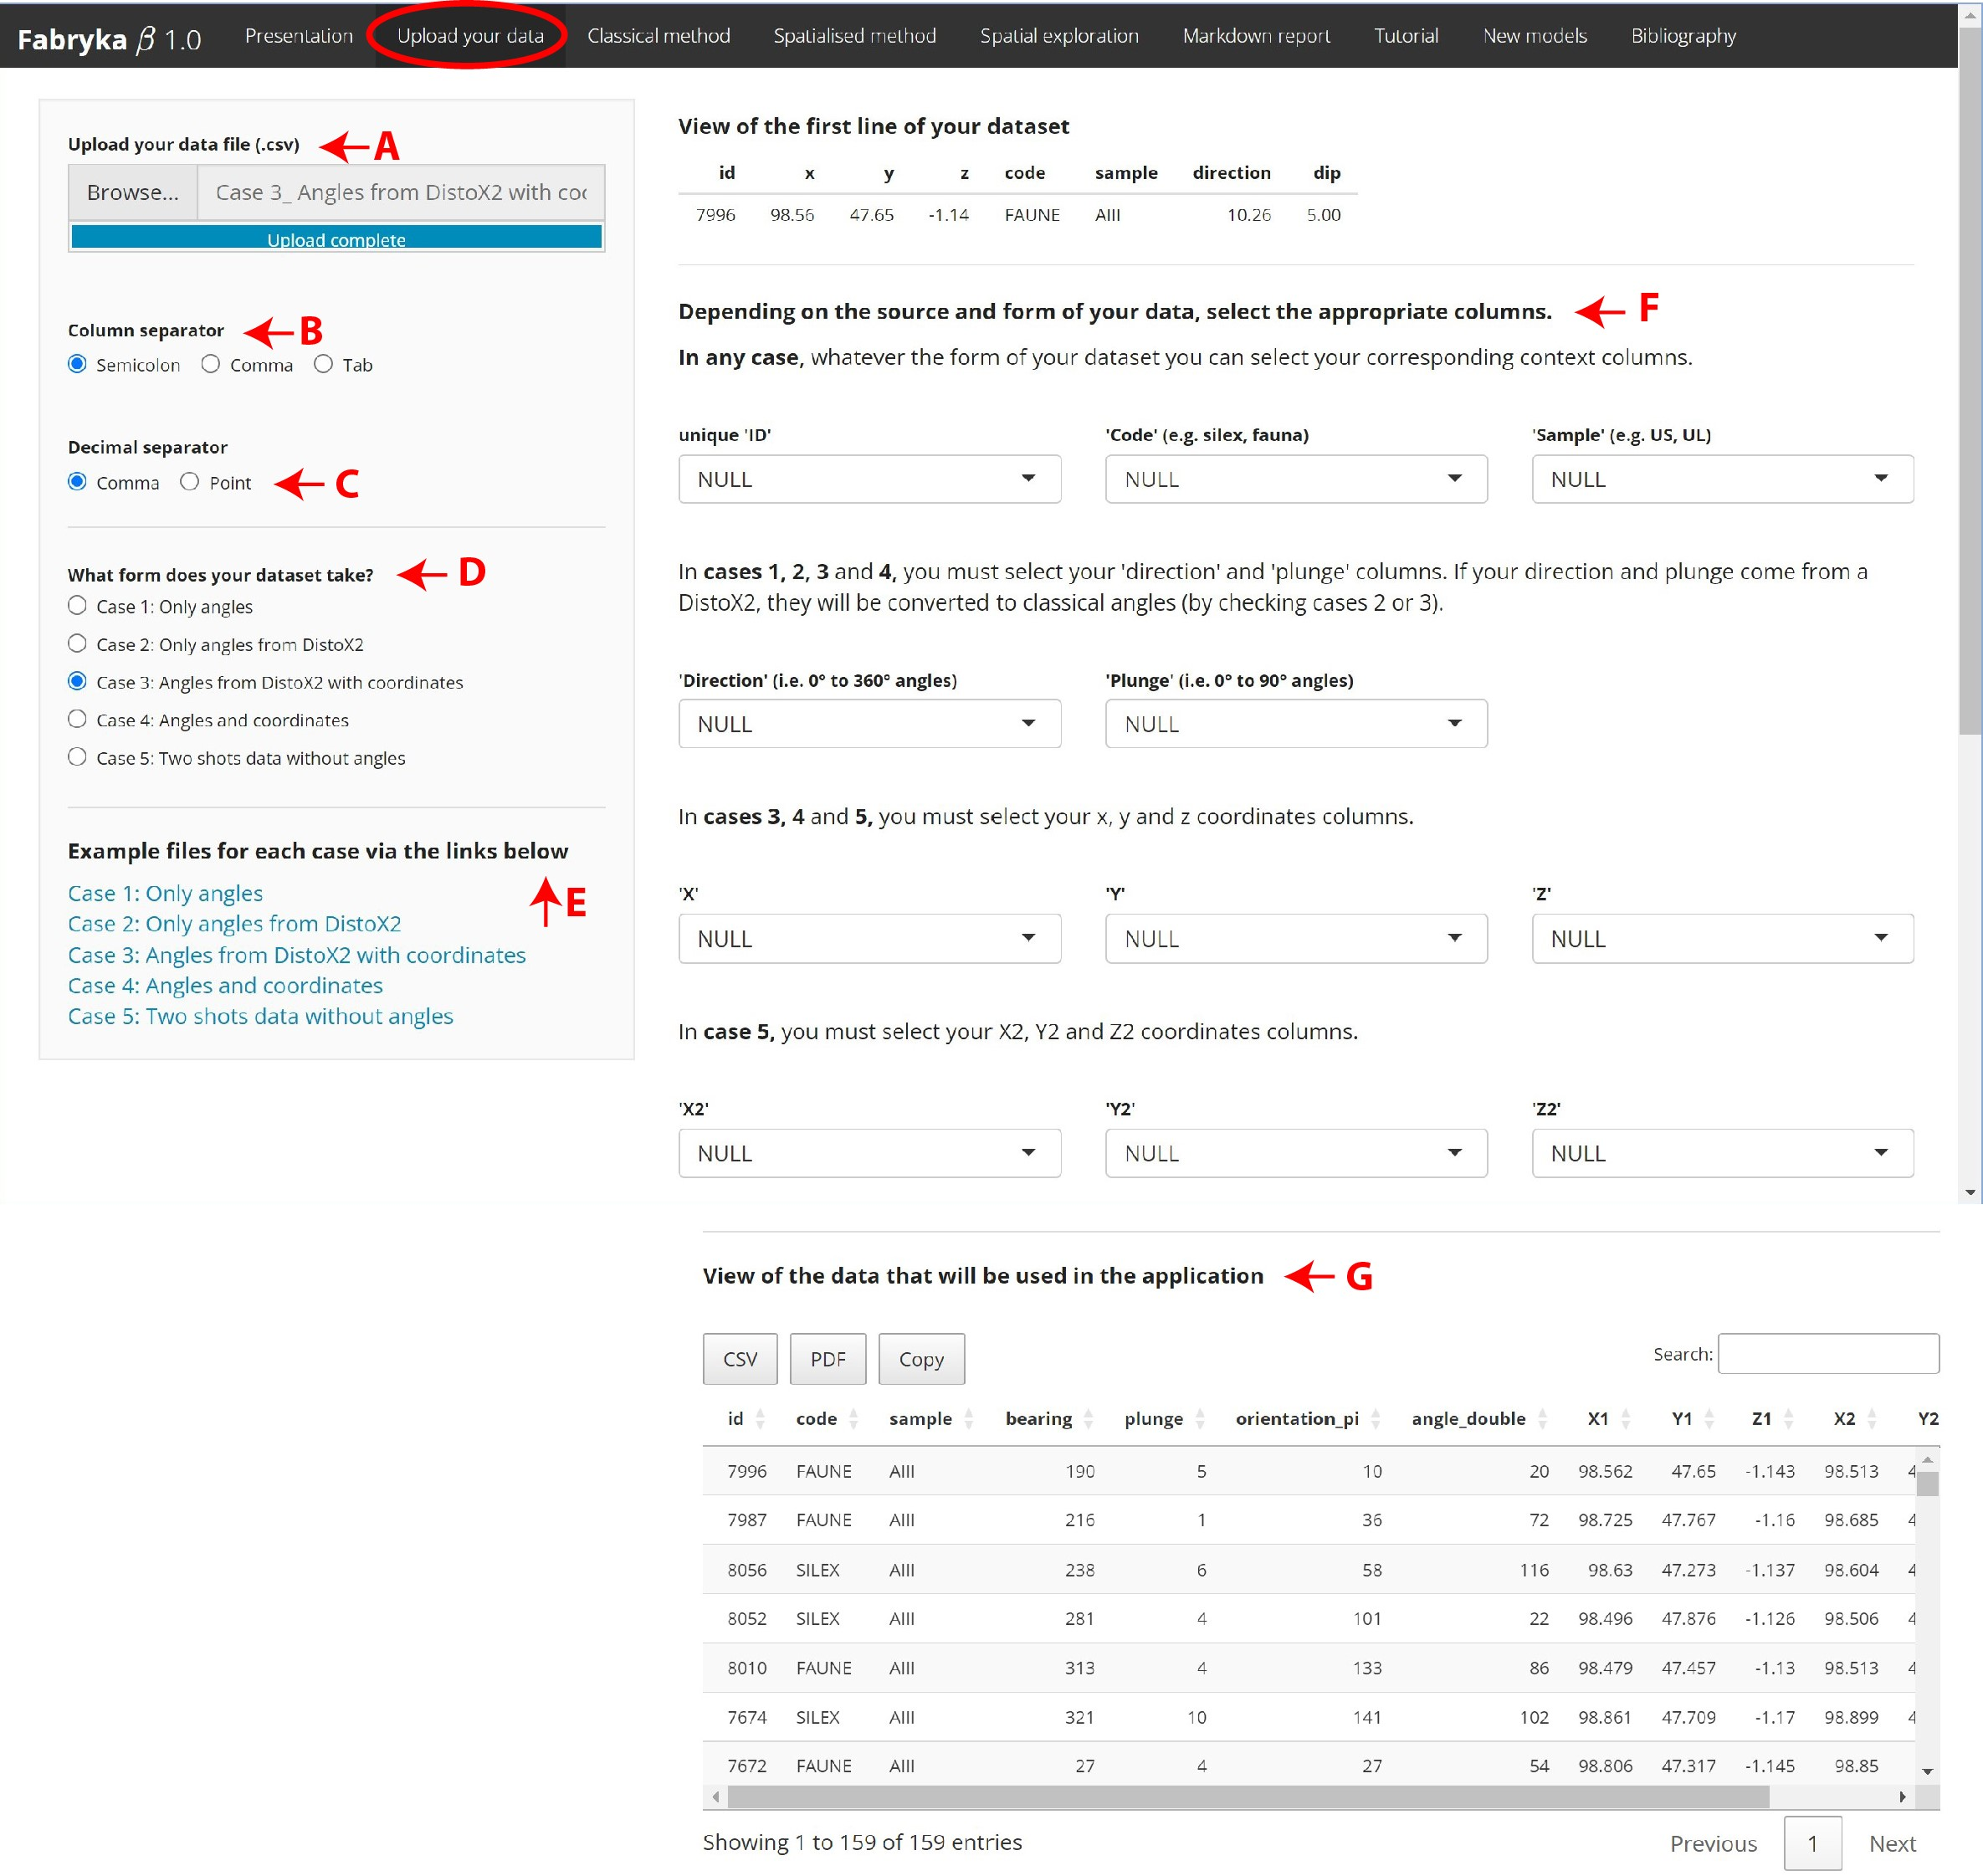
\includegraphics[width=16cm]{figure/upload_your_data.jpg}
  \caption{A. Browse your .csv file, B. choose your column separator, C. choose your decimal separator, D. check the right form of your dataset, E. to do so, have a look of example files, F. select the column needed in the application, G. a new dataset with new columns appears, your are ready to explore your data.}
\label{fig:figure_upload_your_data}
\end{figure}

This panel includes:

\begin{itemize}
\tightlist
\item
  Benn diagrams with possible integration of Bertran and Lenoble
  (\citeproc{ref-bertran2002}{2002}) model (fig.
  \ref{fig:figure_classical_method}D)
\item
  Rose diagrams for axial data and dip (fig.
  \ref{fig:figure_classical_method}G)
\item
  Schmidt diagrams (fig.~\ref{fig:figure_classical_method}H)
\item
  Woodcock diagrams
\item
  Summary data table with Benn indices, additional statistics, and
  orientation statistical tests.
\end{itemize}

In this last table (fig.~\ref{fig:figure_classical_method}I):

\begin{itemize}
\tightlist
\item
  \(N\) stands for number of measures in the samples
\item
  \(E1\), \(E2\) and \(E3\) are the eigenvalues
  (\citeproc{ref-watson1966}{Watson 1966}). They correspond to the sum
  of the cosines formed by the axis of the objects and the three axis of
  the space. They are used to compute the Benn indices
\item
  \(IS\) and \(EL\) are the Benn indices ratios standing respectively
  for, `isotropy' with \(IS = E3/E1\) and `elongation' with
  \(EL = 1-(E2/E1)\) (\citeproc{ref-benn1994}{Benn 1994}).
\item
  \(K\) and \(C\) are the Woodcock (\citeproc{ref-woodcock1977}{1977})
  indices.
\item
  \(L\) is the Vector Magnitude (strength of the preferred orientation)
  and \(R.p\) is the p-value result of the Rayleigh test.
\item
  \(L.double\) and \(R.p.double\) are the same statistics that above for
  double angles (\citeproc{ref-krumbein1939}{Krumbein 1939}).
\item
  \(Rao_p\) is the p\_value of the Rao
  (\citeproc{ref-rao1967large}{1967}) test.
\end{itemize}

You can control the data you plot and the data appearing in the figures
and the summary data table by changing the checkboxes filters (`filter
by sample' and `filter by code') and the slider (\emph{i.e.} minimum
number of measures) in the left sidebar panel (fig.
\ref{fig:figure_classical_method}A, B and C).

\begin{figure} [H]
\centering
  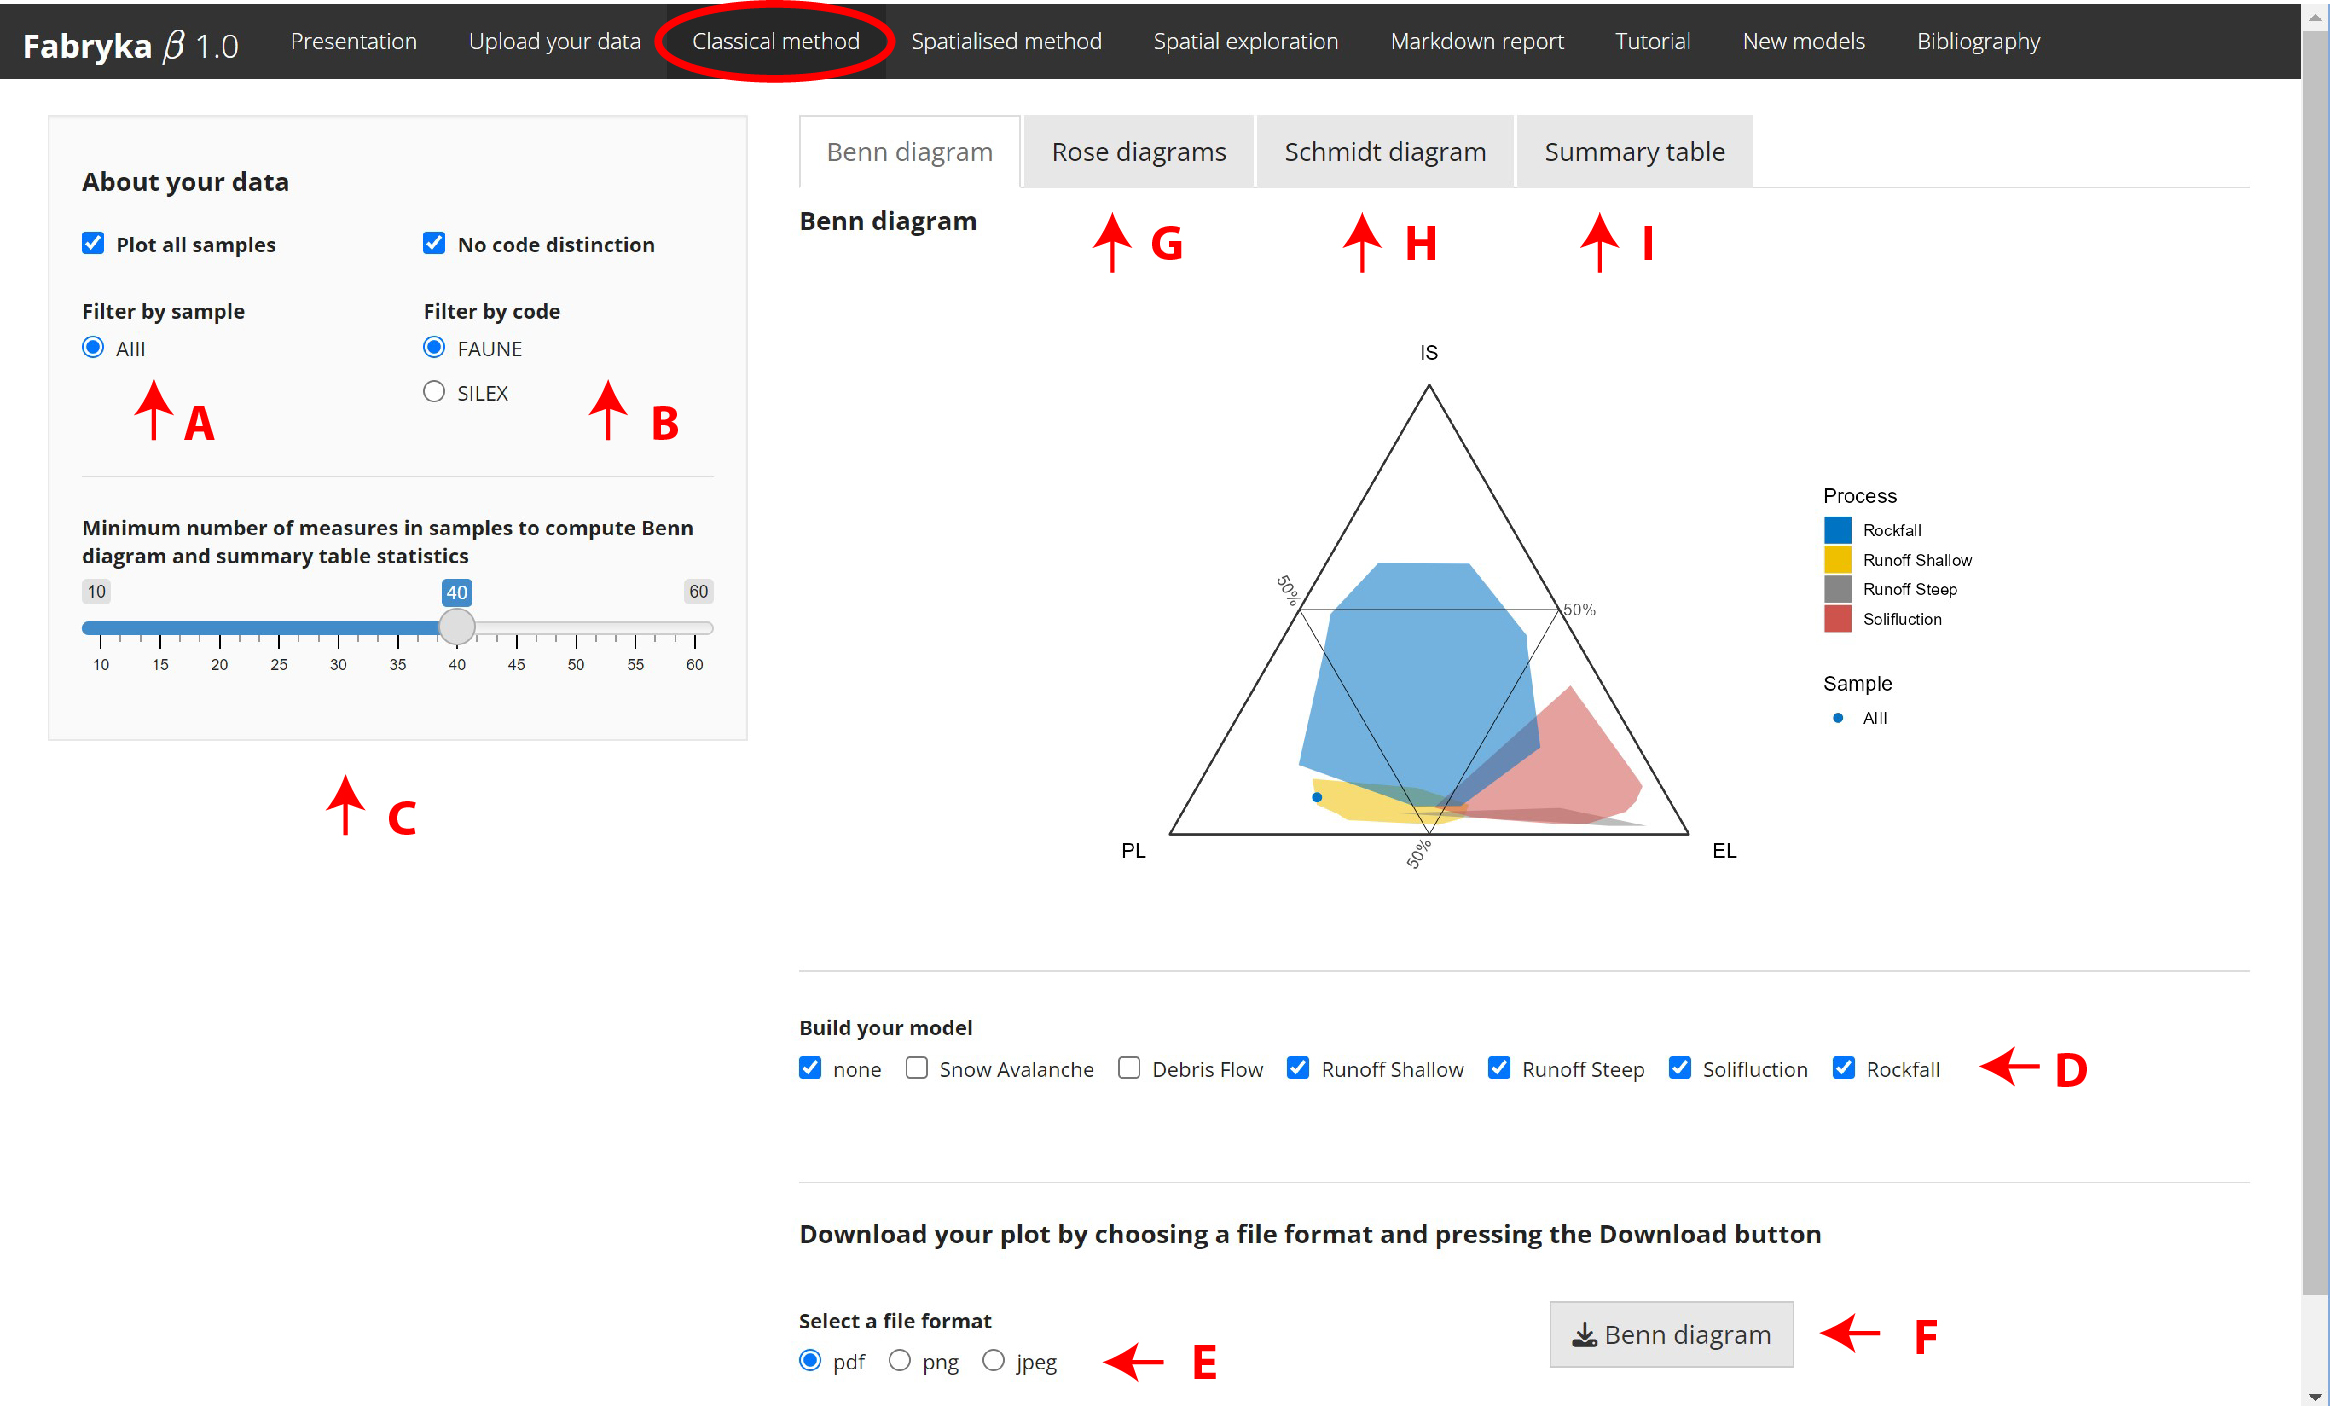
\includegraphics[width=16cm]{figure/classical_method.jpg}
  \caption{A. filter by sample, B. if you want to filter by codes, uncheck 'no code distinction', C. manage the minimum sample size to perform analysis, D. buld your model thanks to Bertran and Lenoble (2002) data, E. and F. download figures by selecting a file format and pressing the 'download' button, G. Rose diagrams subpanel, H. Schmidt diagram subpanel, I. Summary table with additional statistics}
\label{fig:figure_classical_method}
\end{figure}

Certain geological processes can have a different impact on objects
depending on their physical properties (\emph{e.g.} silex versus bones
in a water flow as in the example files provided where bones have a
strong preferential orientation and are much more `linear' in the Benn
diagram (\citeproc{ref-thomas2019}{Thomas et al. 2019};
\citeproc{ref-texier2020}{Texier et al. 2020})). The natural processes
models that you can add to the Benn diagram are calculated using data
mainly from (\citeproc{ref-bertran1997}{Bertran et al. 1997},
\citeproc{ref-bertran2006}{2006}; \citeproc{ref-bertran2002}{Bertran and
Lenoble 2002}; \citeproc{ref-lenoble2004}{Lenoble and Bertran 2004}).
You will find the reference model data (with corresponding literature
references) which is used in the application in the `Model reference
data' subpanel. In the rose diagram, axial data is considered (and not
orientations) as the Rayleigh test is perform on axial data
(\citeproc{ref-curray1956}{Curray 1956}) in the summary table. You can
download all the figures by selecting a file format (.pdf, .jpeg and
.png) and pressing the `download' button (fig.
\ref{fig:figure_classical_method}E and F).

\subsection{Spatialised method}\label{spatialised-method-1}

This panel includes (fig.~\ref{fig:figure_spatialised_method}):

\begin{itemize}
\tightlist
\item
  Benn diagrams with Benn indices computed with nearest neighbors points
  (\citeproc{ref-mcpherron2018}{S. P. McPherron 2018})
\item
  Spatial projections of the points according to their fabric shape
\item
  Summary data tables with orientation statistical tests, one at the
  scale of each spatial series (each object and its \(n\) nearest
  neighbors fabric = one row) and one at the scale of the sample (fig.
  \ref{fig:figure_spatialised_method}F and G).
\end{itemize}

A table similar to the one done in the Classical method is proposed and
contains the same statistics .

At the spatial series scale (\emph{i.e.} each points and \(n\)
neighbors), statistics are provided in a table (Spatial series data
table subpanel) with the Benn indices, the orientation rates \(L\),
\(L.double\) and \(p-values\) returned by the Rayleigh tests. At the
sample scale, mean and standard deviations values of Benn indices, mean
\(L\) and its corresponding Rayleigh tests means (mean values of all
spatial series in the sample) and rejections ratios \(Tr\) (formula
\textbf{4.}) are given in the subpanel `Summary table of samples'.

In the projections, the orientation of the objects can be materialized
by sticks (by unchecking the corresponding box in the left sidebar
panel, fig.~\ref{fig:figure_spatialised_method}D) which color is
representative of the fabric of the series formed by the object and its
\(n\) nearest neighbors. You can also add orthophoto in the background
of projections (fig.~\ref{fig:figure_spatialised_method}E). In the left
sidebar panel, you can control the samples considered in the analysis by
selecting the sample explored or by distinguishing the code used
(\emph{e.g.} flint versus bone,
fig.~\ref{fig:figure_spatialised_method}A and B). You can also use the
slider to change the number of neighbors searched for around each point
(fig.~\ref{fig:figure_spatialised_method}C). Be careful, this will alter
the results obtained in the Benn diagram and Rayleigh tests. \bigbreak

\subsection{Spatial exploration}\label{spatial-exploration}

This panel includes (fig.~\ref{fig:figure_spatial_exploration}):

\begin{itemize}
\tightlist
\item
  A spatial exploration of your data starting from a Benn diagram
\item
  A spatial exploration of your data starting from the spatial
  projections (fig.~\ref{fig:figure_spatial_exploration}J)
\item
  Summary data tables with orientation statistical tests (fig.
  \ref{fig:figure_spatial_exploration}I and K).
\end{itemize}

In this panel, you can perform a spatial analysis of your data starting
from a Benn diagram or from projections. In both cases, you need to
select the data you want to explore more locally in a new analysis. From
the projections, you can select the points you want to explore directly.
In the Benn diagram, you need to select the lasso selector (fig.
\ref{fig:figure_spatial_exploration}D). Pay attention to the number of
points selected and check that the new sample contains enough points to
carry out the new analysis. If this is not the case, you can lower the
slider in the left sidebar panel to perform the analysis with fewer
neighbors (fig.~\ref{fig:figure_spatial_exploration}E). You can download
the new samples you have selected with spatial statistics from the
corresponding subpanels (fig.~\ref{fig:figure_spatial_exploration}I and
K). \bigbreak

\begin{figure} [h]
\centering
  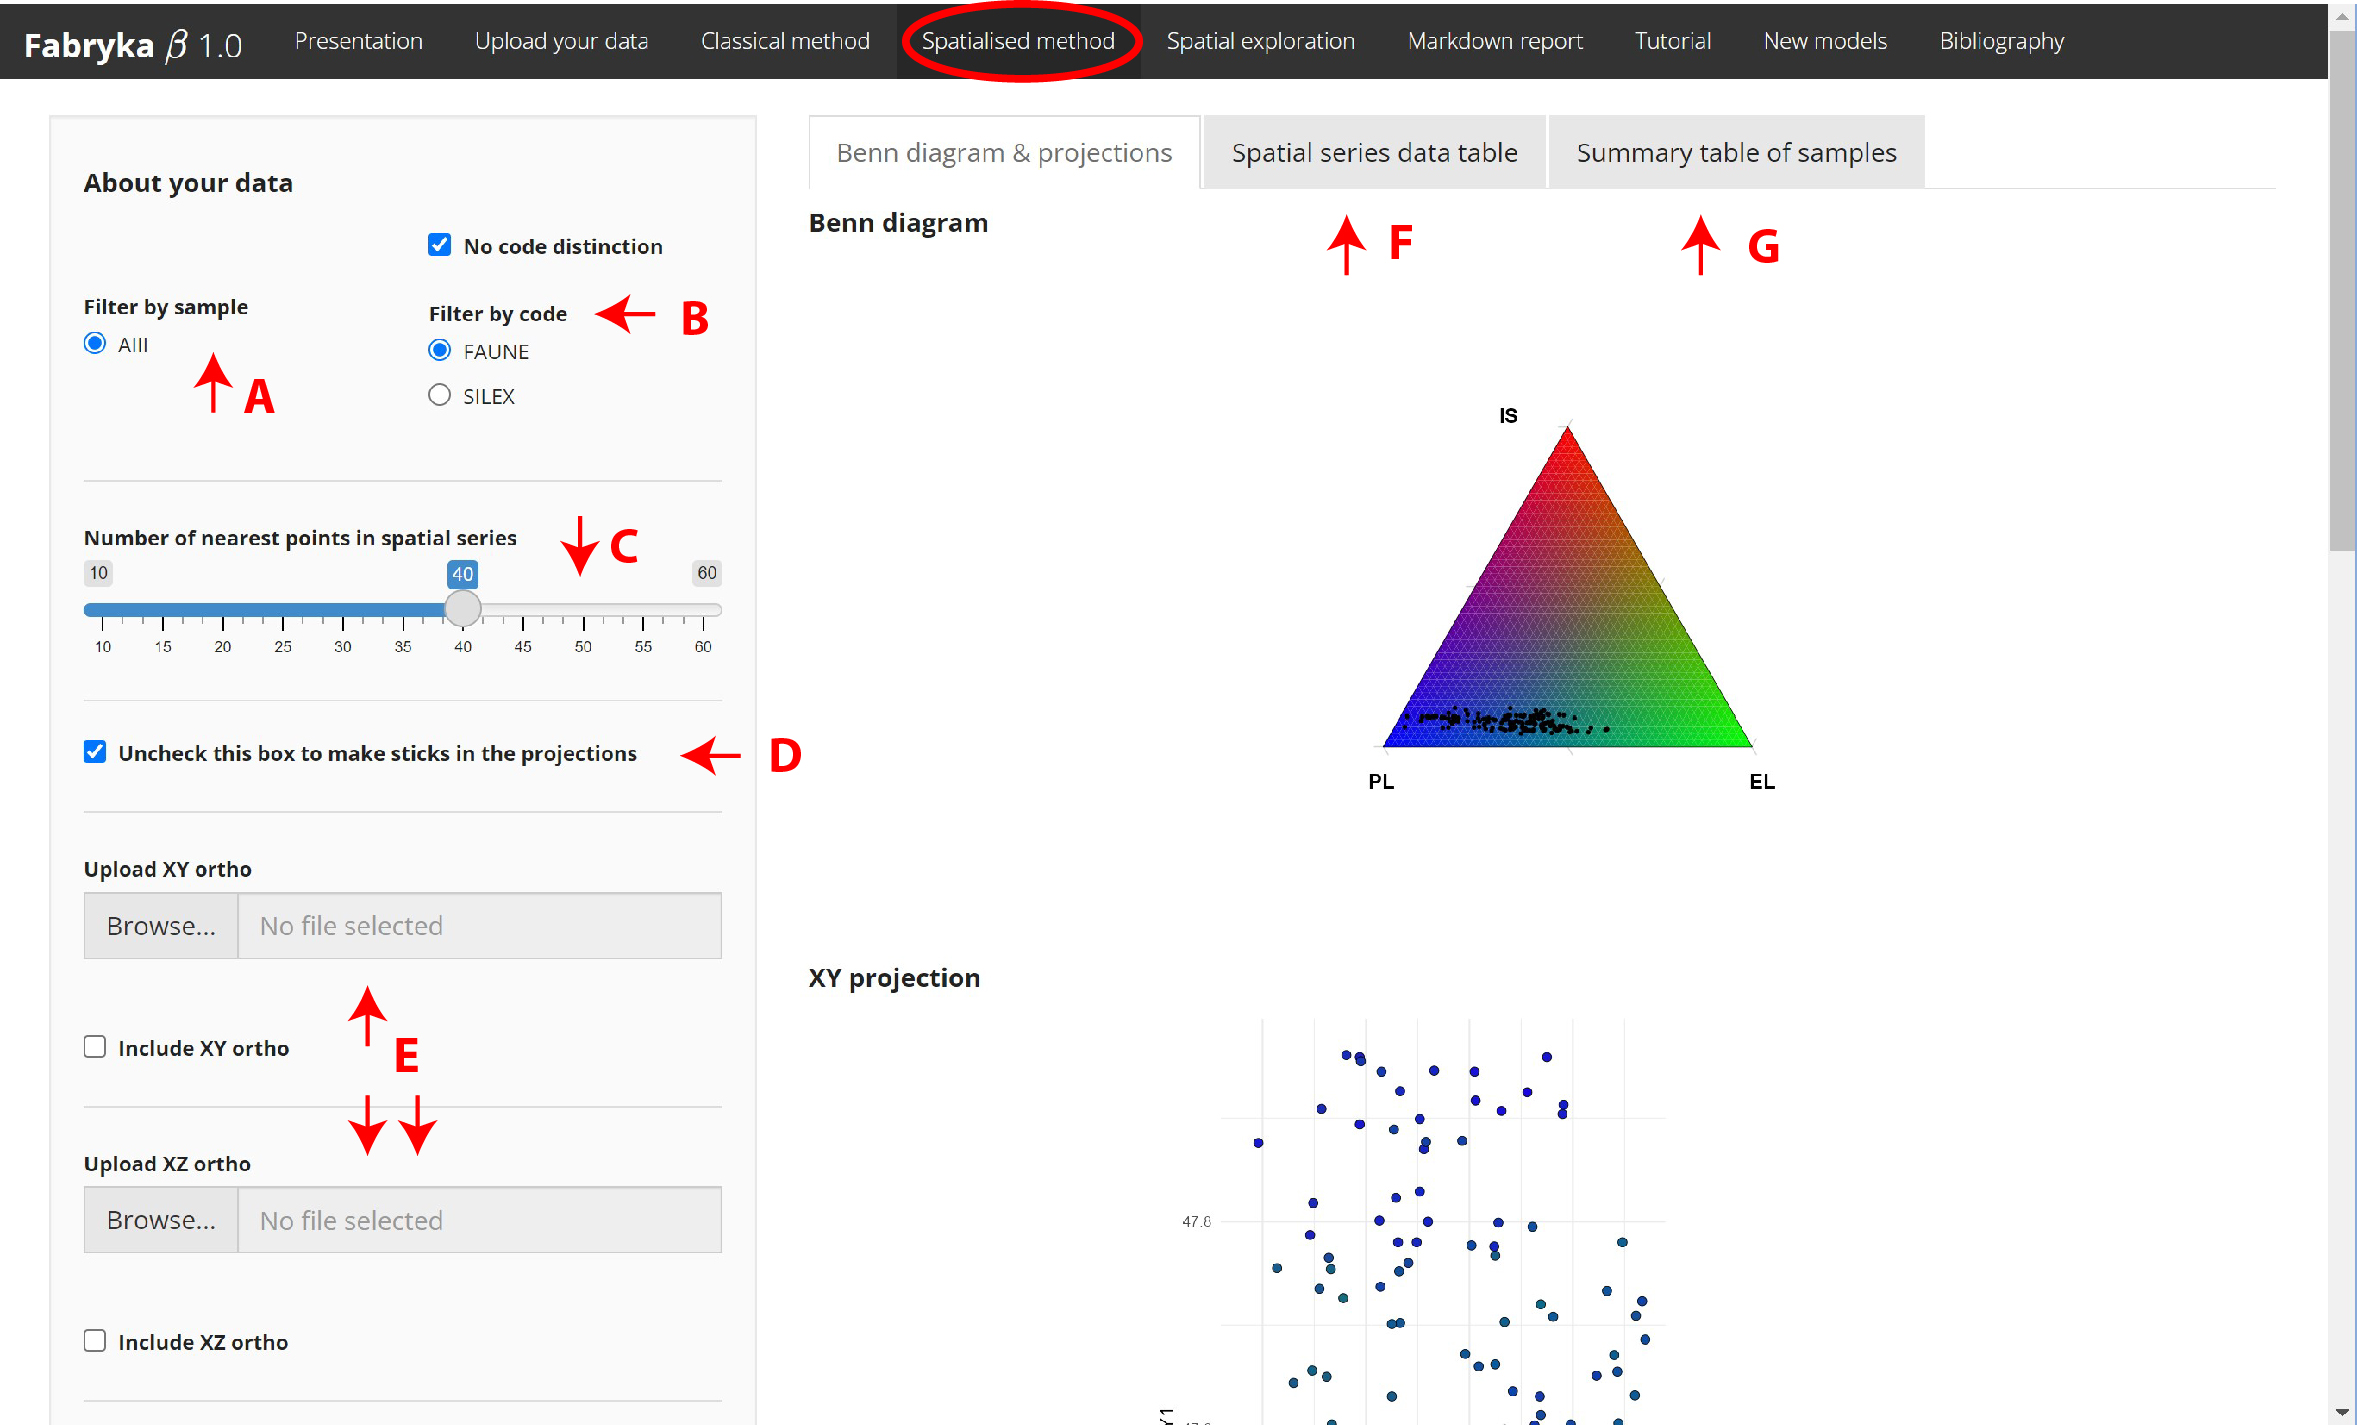
\includegraphics[width=16cm]{figure/spatialised_method.jpg}
  \caption{A. filter by sample, B. if you want to filter by code, uncheck 'no code distinction', C. choose the n nearest neighbors to perform the statistics, D. make sticks in spatial projections, E. upload a georeferenced orthophoto and check 'include' orthophoto to display it, F. new dataset at the spatial series scale, G. summary table at the sample scale.}
\label{fig:figure_spatialised_method}
\end{figure}

\subsection{Tutorial}\label{tutorial}

The `Tutorial' panel contains a summary of the mathematics, statistics
and methods used in fabryka and a short tutorial directly accessible
from the application. \bigbreak

\begin{figure} [h]
\centering
  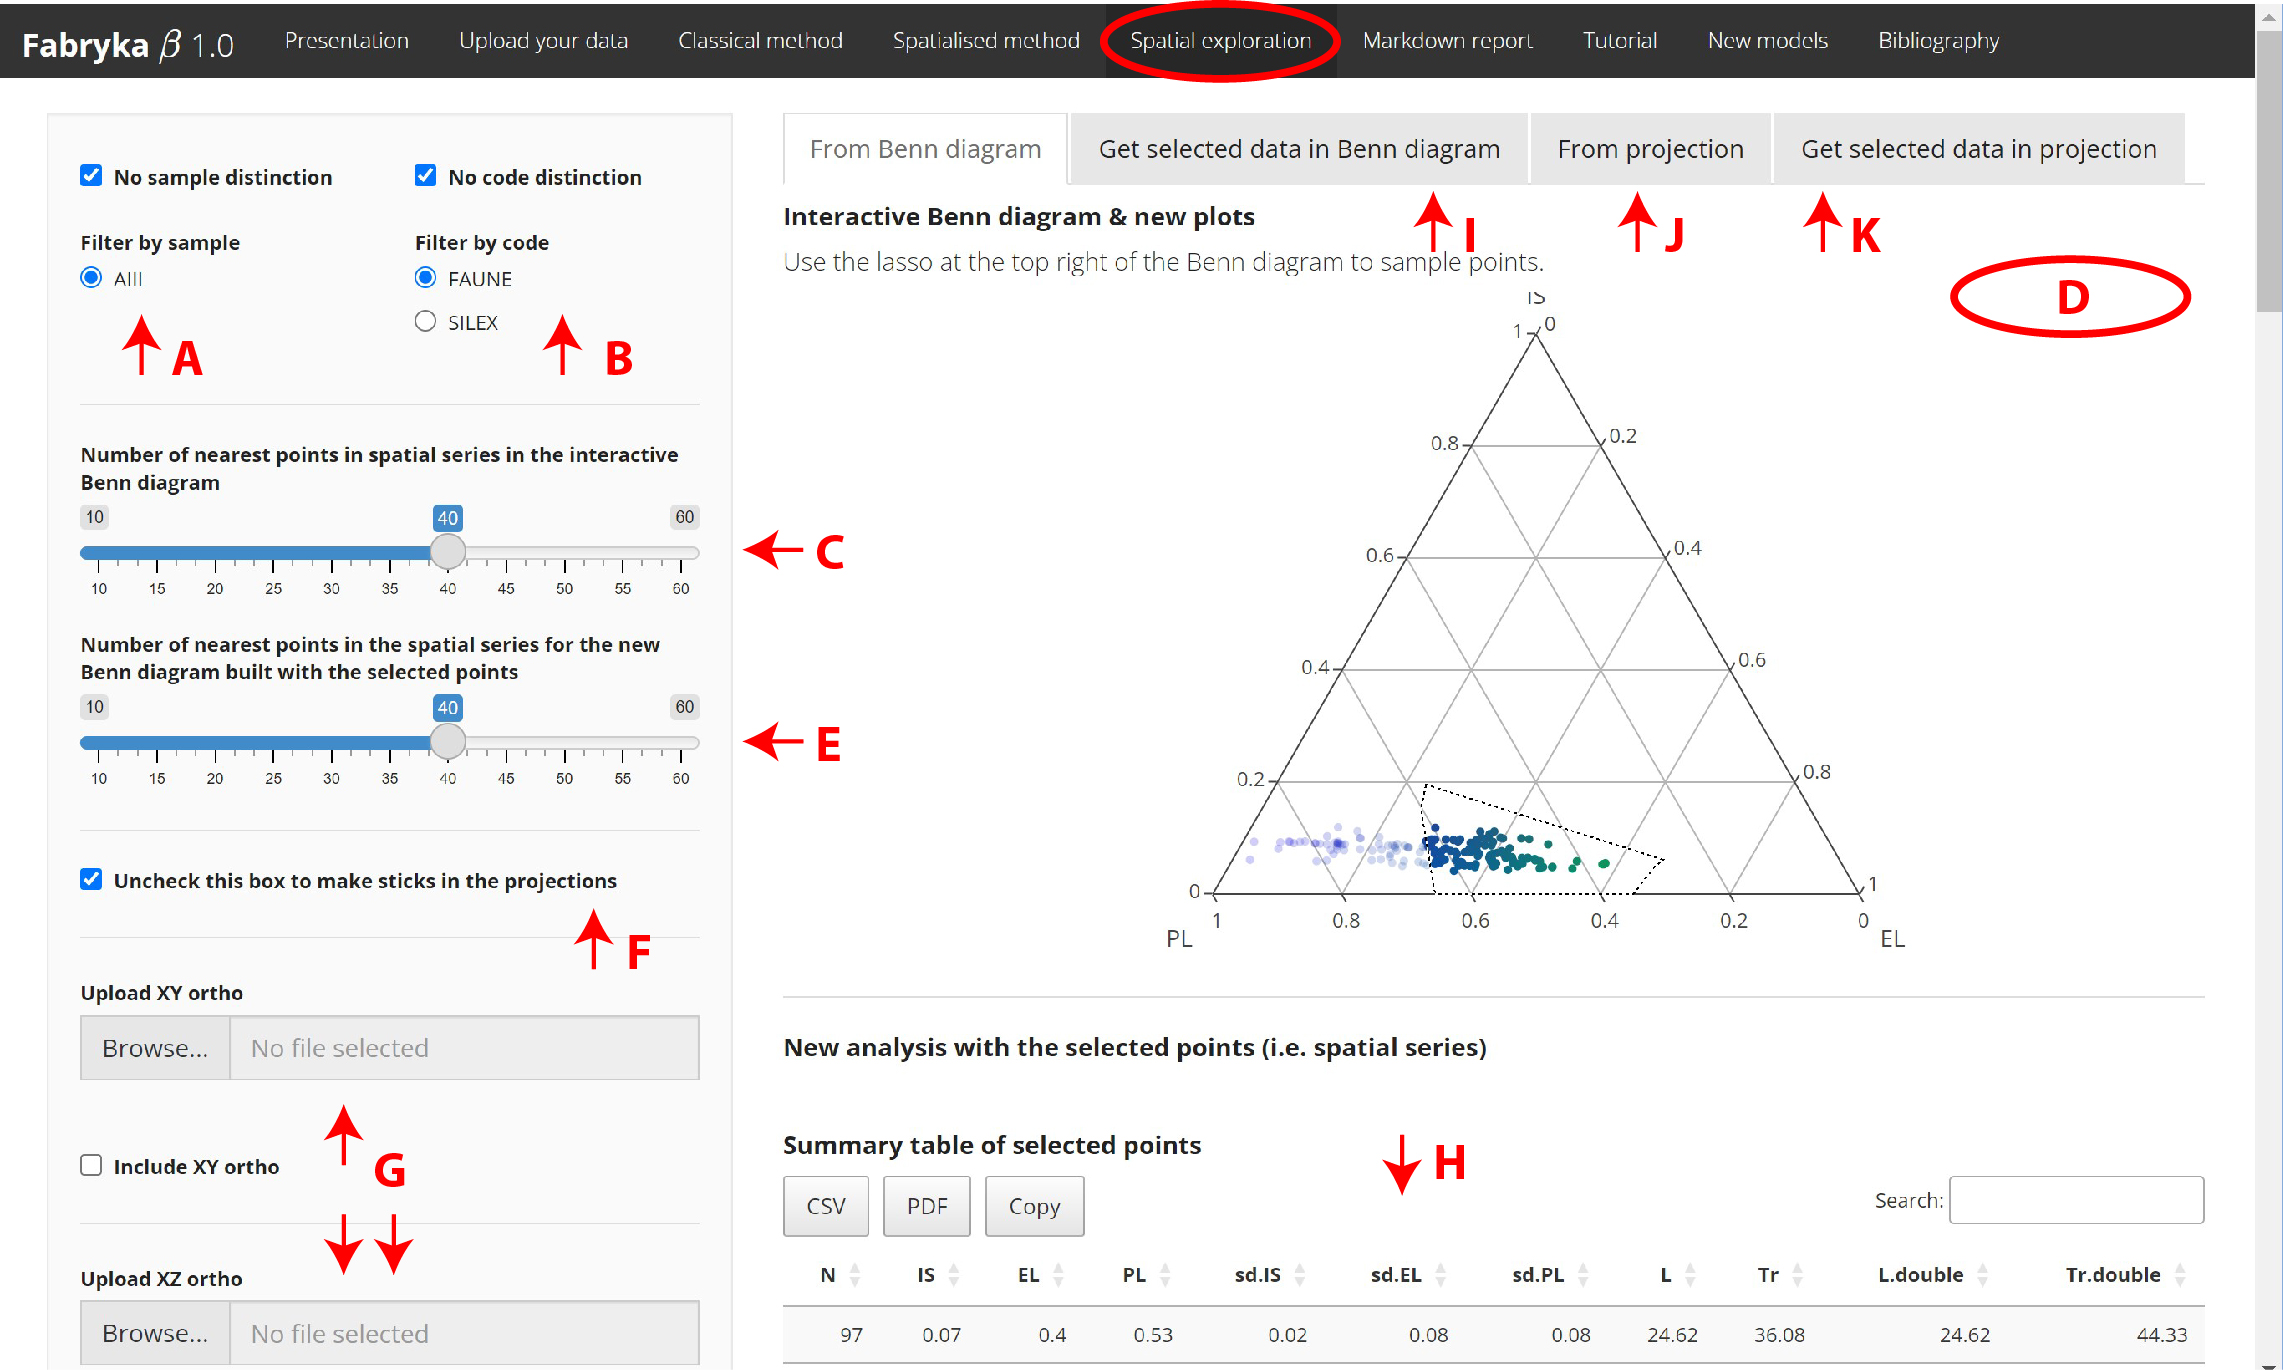
\includegraphics[width=16cm]{figure/spatial_exploration.jpg}
  \caption{A. if you want to filter by sample, uncheck 'No sample distinction' B. if you want to filter by code, uncheck 'no code distinction', C. choose the n nearest neighbors to perform the statistics (first Benn diagram), E. choose the n nearest neighbors to perform the statistics on the sampled data (second Benn diagram), F. make sticks in spatial projections, G. you can upload a georeferenced orthophoto and check 'include' orthophoto to display it, H. a new spatial exploration of the fabric is performed, I. new dataset at the selected spatial series scale, I. a similar spatial exploration is possible from the projections, K. new dataset at the selected spatial series scale.}
\label{fig:figure_spatial_exploration}
\end{figure}

\subsection{New reference models}\label{new-reference-models}

The `spatialised' method generates often more linear fabrics in
comparison with the `classical' method. This can be explained by the
fact that objects that are close in space are more likely to resemble
each other than objects that are further in space. A difference between
global fabric (``classical method'', \emph{i.e.}, one point per sample)
and spatialised fabric (series of n neighbors) in Benn diagrams marks a
spatial heterogeneity that needs to be explored.

Also, the structure of the point pattern is evocative of its fabric.
Thus, the dispersion of the points depends on the shape of the fabric.
Two extremes appear: the most isotropic samples are those with the most
dispersed point patterns (\emph{i.e.} the standard deviations are high)
while the most linear samples are those with the least dispersed point
patterns. Planar samples highlight point patterns with intermediate
dispersion. The explanation of this phenomenon is intuitive: the more
similar the fabrics of objects are, the closer they are in the Benn
diagram and the more linear they are. To reflect this phenomenon, the
standard deviations of the Benn indices are calculated and aim to
describe the dispersion point patterns in the Benn diagrams.

Global planar or isotropic fabrics can sometimes mask local anisotropy.
Within certain samples, groups of objects form a dense cluster in the
point pattern. This is expressed either by a locally more linear fabric,
or by a planar fabric with a strong bimodal orientation.

For the reasons given above, we wish to create new models that
considered the particularities of the spatial method. A panel was
therefore set up to collect new data describing the fabric of
sedimentary processes in order to build a new ``spatialised'' reference
model (\emph{cf.} the ``classical'' model proposed by Bertran and
Lenoble (\citeproc{ref-bertran2002}{2002})). This work is in progress.
This panel will be updated in the next version of the application.

\bigbreak

\subsection{Contributors}\label{contributors}

The contributors panel aims at citing all contributors of this project.
\bigbreak

\section{Data, scripts, code, and supplementary information
availability}\label{data-scripts-code-and-supplementary-information-availability}

\begin{itemize}
\tightlist
\item
  use fabryka online: \url{https://marchaeologist.shinyapps.io/fabryka/}
  \smallbreak
\item
  source code: \url{https://github.com/marchaeologist/fabryka/tree/main}
  \smallbreak
\item
  Report bugs or any request:
  \url{https://github.com/marchaeologist/fabryka/issues} \smallbreak
\item
  github reprository doi of fabryka:
  \url{https://doi.org/10.5281/zenodo.15909666} \smallbreak
\item
  Zenodo repository of this article:
  \url{https://doi.org/10.5281/zenodo.16758152} \bigbreak
\end{itemize}

\textbf{If you are preparing a mission in a field without Internet
access:}

\begin{enumerate}
\def\labelenumi{\arabic{enumi}.}
\item
  Install \href{https://www.r-project.org}{R} and
  \href{https://posit.co/download/rstudio-desktop/}{Rstudio Desktop}.
\item
  Clone the fabryka repository from GitHub:
  \url{https://github.com/marchaeologist/fabryka} or download the code
  in ``Code'' and ``Download ZIP'' at the same address. Unzip the
  folder. This will give you the latest version of the source code.
\item
  Open fabryka.Rproj
\item
  If you are using the application for the first time, you have to
  install several packages used in the application. Lists of all these
  packages and dependencies are available in a DESCRIPTION file and a
  DEPENDECIES file in the github repository. To install fabryka packages
  and dependencies, copy and paste the following code lines into the R
  console:
\end{enumerate}

\begin{Shaded}
\begin{Highlighting}[]
\NormalTok{fabryka\_packages }\OtherTok{=} \FunctionTok{c}\NormalTok{(}\StringTok{"shiny"}\NormalTok{, }\StringTok{"dplyr"}\NormalTok{,}\StringTok{"ggplot2"}\NormalTok{,}\StringTok{"plotly"}\NormalTok{, }\StringTok{"ggsci"}\NormalTok{, }\StringTok{"ggtern"}\NormalTok{, }\StringTok{"circular"}\NormalTok{, }
                     \StringTok{"CircStats"}\NormalTok{, }\StringTok{"Ternary"}\NormalTok{, }\StringTok{"RStoolbox"}\NormalTok{, }\StringTok{"shinyjs"}\NormalTok{, }\StringTok{"rmarkdown"}\NormalTok{, }
                     \StringTok{"shinythemes"}\NormalTok{,  }\StringTok{"ggalt"}\NormalTok{, }\StringTok{"DT"}\NormalTok{, }\StringTok{"raster"}\NormalTok{)}

\NormalTok{is\_installed }\OtherTok{=} \FunctionTok{sapply}\NormalTok{(fabryka\_packages, require, }\AttributeTok{character.only=}\NormalTok{T)}

\FunctionTok{sapply}\NormalTok{(fabryka\_packages[}\SpecialCharTok{!}\NormalTok{is\_installed], install.packages)}
\end{Highlighting}
\end{Shaded}

\begin{enumerate}
\def\labelenumi{\arabic{enumi}.}
\setcounter{enumi}{4}
\tightlist
\item
  The application can be launched by opening the app.R file in the main
  folder and pressing ``Run App'' or by running the following commands:
\end{enumerate}

\begin{Shaded}
\begin{Highlighting}[]
\NormalTok{pkgload}\SpecialCharTok{::}\FunctionTok{load\_all}\NormalTok{(}\StringTok{"."}\NormalTok{)}

\FunctionTok{fabryka}\NormalTok{()}
\end{Highlighting}
\end{Shaded}

\section{Acknowledgements}\label{acknowledgements}

The writing of the script was greatly facilitated by the work published
by Shannon McPherron (2018). It includes some functions published by the
author, with a few modifications. This work benefited from discussions
with Jean-Pierre Texier, Arnaud Lenoble, Pascal Bertran, Thomas Perrin
and Dominique Todisco on issues related to site formation processes. The
reference data used to build the models of the classical method were
collected by P. Bertran throughout his career. Pascal Bertran provided
us with all these data in order to feed the application. The development
of the application also benefited from the help of Rémi Lemoy, François
Baleux and Victor Baleux on mathematical issues. A first version of the
application was tested by Emmanuel Discamps and Aurélien Royer. This
project is supported by the ``Service Valorisarion de la Recherche'' of
the University Toulouse Jean Jaurès. A preprint version of this article
(v3, \url{https://doi.org/10.5281/zenodo.16601423}) has been
peer-reviewed and recommended by PCI Archaeo
(\url{https://doi.org/10.24072/pci.archaeo.100611}). Comments made by
Pascal Bertran, recommender of this article, and, by Frédéric Santos,
Nicolas Frerebeau and Alfonso Benito-Calvo, reviewers of this article,
considerably improved the manuscript and the application. I would like
to thank all these reasearchers for their advice. \bigbreak

\section{Funding}\label{funding}

This research was funded by the Service Valorisation de la Recherche of
Toulouse - Jean Jaurès University. \bigbreak

\section{Conflict of interest
disclosure}\label{conflict-of-interest-disclosure}

The authors declare that they comply with the PCI rule of having no
financial conflicts of interest in relation to the content of the
article. \bigbreak

\section{References}\label{references}

The `Bibliography' panel in the application contains the references
cited in the application. This article contains the same bibliography
with some additional references. \bigbreak

\phantomsection\label{refs}
\begin{CSLReferences}{1}{0}
\bibitem[\citeproctext]{ref-allaire2014}
Allaire, Joseph J, Yihui Xie, Christophe Dervieux, Jonathan McPherson,
Javier Luraschi, Kevin Ushey, Aron Atkins, et al. 2014. {``Rmarkdown:
Dynamic Documents for r.''} \emph{(No Title)}.

\bibitem[\citeproctext]{ref-benn1994}
Benn, Douglas. 1994. {``Fabric Shape and the Interpretation of
Sedimentary Fabric Data.''} \emph{Journal of Sedimentary Research} 64
(4a): 910915.

\bibitem[\citeproctext]{ref-bertran2006}
Bertran, Pascal, Jean-Guillaume Bordes, Antoine Barré, Arnaud Lenoble,
and Vincent Mourre. 2006. {``Fabrique d'amas de Débitage: Données
Expérimentales.''} \emph{Bulletin de La Société Préhistorique
Française}, 3347.

\bibitem[\citeproctext]{ref-bertran1997}
Bertran, Pascal, Bernard Hetu, Jean-Pierre Texier, and Henk Van Steijn.
1997. {``Fabric Characteristics of Subaerial Slope Deposits.''}
\emph{Sedimentology} 44 (1): 116.

\bibitem[\citeproctext]{ref-bertran2002}
Bertran, Pascal, and Arnaud Lenoble. 2002. {``Fabriques Des Niveaux
Archéologiques: Méthode Et Premier Bilan Des Apports à l{'}étude
Taphonomique Des Sites Paléolithiques.''} \emph{PALEO. Revue
d'archéologie Préhistorique}, no. 14: 1328.

\bibitem[\citeproctext]{ref-chang2024}
Chang, Winston, Joe Cheng, J. J. Allaire, Carson Sievert, Barret
Schloerke, Yihui Xie, Jeff Allen, Jonathan McPherson, Alan Dipert, and
Barbara Borges. 2024. \emph{Shiny: Web Application Framework for r}.
\url{https://CRAN.R-project.org/package=shiny}.

\bibitem[\citeproctext]{ref-curray1956}
Curray, Joseph R. 1956. {``The Analysis of Two-Dimensional Orientation
Data.''} \emph{The Journal of Geology} 64 (2): 117131.

\bibitem[\citeproctext]{ref-discamps2024}
Discamps, Emmanuel, Marc Thomas, Jean-Philippe Faivre, and Brad Gravina.
2024. {``Protocole de Fouille Sur Les Sites Paléolithiques:
Justification Des Besoins Et Modalités de Mise En Øeuvre à Combe-Grenal
Et à l{'}abri Inférieur Du Moustier (Dordogne, France).''} \emph{Gallia
Préhistoire}, no. 64.

\bibitem[\citeproctext]{ref-isaac1967}
Isaac, Glynn L. 1967. {``Towards the Interpretation of Occupation
Debris: Some Experiments and Observations.''} \emph{Kroeber
Anthropological Society Papers} 37 (37): 3157.

\bibitem[\citeproctext]{ref-krumbein1939}
Krumbein, William C. 1939. {``Preferred Orientation of Pebbles in
Sedimentary Deposits.''} \emph{The Journal of Geology} 47 (7): 673706.

\bibitem[\citeproctext]{ref-lenoble2004}
Lenoble, Arnaud, and Pascal Bertran. 2004. {``Fabric of Palaeolithic
Levels: Methods and Implications for Site Formation Processes.''}
\emph{Journal of Archaeological Science} 31 (4): 457469.

\bibitem[\citeproctext]{ref-mcpherron2005artifact}
McPherron, Shannon JP. 2005. {``Artifact Orientations and Site Formation
Processes from Total Station Proveniences.''} \emph{Journal of
Archaeological Science} 32 (7): 1003--14.

\bibitem[\citeproctext]{ref-mcpherron2018}
McPherron, Shannon P. 2018. {``Additional Statistical and Graphical
Methods for Analyzing Site Formation Processes Using Artifact
Orientations.''} \emph{PloS One} 13 (1): e0190195.

\bibitem[\citeproctext]{ref-rao1967large}
Rao, JS. 1967. {``Large Sample Tests for the Homogeneity of Angular
Data.''} \emph{Sankhya Ser B} 28: 172--74.

\bibitem[\citeproctext]{ref-sanchez2016assessment}
Sánchez-Romero, Laura, Alfonso Benito-Calvo, Alfredo Pérez-González, and
Manuel Santonja. 2016. {``Assessment of Accumulation Processes at the
Middle Pleistocene Site of Ambrona (Soria, Spain). Density and
Orientation Patterns in Spatial Datasets Derived from Excavations
Conducted from the 1960s to the Present.''} \emph{PloS One} 11 (12):
e0167595.

\bibitem[\citeproctext]{ref-schick1986}
Schick, Kathy Diane. 1986. {``Stone Age Sites in the Making: Experiments
in the Formation and Transformation of Archaeological Occurrences.''}
\emph{(No Title)}.

\bibitem[\citeproctext]{ref-schiffer1983}
Schiffer, Michael B. 1983. {``Toward the Identification of Formation
Processes.''} \emph{American Antiquity} 48 (4): 675706.

\bibitem[\citeproctext]{ref-rcoreteam2025}
Team, R Core. 2025. \emph{R: A Language and Environment for Statistical
Computing}. Vienna, Austria: R Foundation for Statistical Computing.
\url{https://www.R-project.org/}.

\bibitem[\citeproctext]{ref-texier2020}
Texier, Jean-Pierre, Emmanuel Discamps, Brad Gravina, and Marc Thomas.
2020. {``Les Dépôts de Remplissage de l{'}abri Inférieur Du Moustier
(Dordogne, France): Lithostratigraphie, Processus de Formation Et
Évolution Du Système Géomorphologique.''} \emph{PALEO. Revue
d'archéologie Préhistorique}, no. 30-2: 320345.

\bibitem[\citeproctext]{ref-thomas2019}
Thomas, Marc, Emmanuel Discamps, Brad Gravina, and Jean-Pierre Texier.
2019. {``Analyse Taphonomique Et Spatiale de Palimpsestes d'occupations
Moustériennes de l'abri Inférieur Du Moustier (Dordogne, France).''}
\emph{PALEO. Revue d'archéologie Préhistorique}, no. 30-1: 278299.

\bibitem[\citeproctext]{ref-de2013application}
Torre, Ignacio de la, and Alfonso Benito-Calvo. 2013. {``Application of
GIS Methods to Retrieve Orientation Patterns from Imagery; a Case Study
from Beds i and II, Olduvai Gorge (Tanzania).''} \emph{Journal of
Archaeological Science} 40 (5): 2446--57.

\bibitem[\citeproctext]{ref-de2021new}
Torre, Ignacio de la, Alfonso Benito-Calvo, Carmen Martin-Ramos, Lindsay
J McHenry, Rafael Mora, Jackson K Njau, Michael C Pante, Ian G
Stanistreet, and Harald Stollhofen. 2021. {``New Excavations in the MNK
Skull Site, and the Last Appearance of the Oldowan and Homo Habilis at
Olduvai Gorge, Tanzania.''} \emph{Journal of Anthropological
Archaeology} 61: 101255.

\bibitem[\citeproctext]{ref-watson1966}
Watson, Geoffrey S. 1966. {``The Statistics of Orientation Data.''}
\emph{The Journal of Geology} 74 (5, Part 2): 786797.

\bibitem[\citeproctext]{ref-woodcock1977}
Woodcock, NH. 1977. {``Specification of Fabric Shapes Using an
Eigenvalue Method.''} \emph{Geological Society of America Bulletin} 88
(9): 12311236.

\bibitem[\citeproctext]{ref-xie2018}
Xie, Yihui, Joseph J Allaire, and Garrett Grolemund. 2018. \emph{R
Markdown: The Definitive Guide}. Chapman; Hall/CRC.

\bibitem[\citeproctext]{ref-xie2020}
Xie, Yihui, Christophe Dervieux, and Emily Riederer. 2020. \emph{R
Markdown Cookbook}. Chapman; Hall/CRC.

\end{CSLReferences}

\end{document}
